%%% Choose between 16:9 and 4:3 format by commenting out/uncommenting one of the following lines:
 \documentclass[aspectratio=169]{beamer} % 16:9
%\documentclass{beamer} % 4:3

%=========================================================================================================================

\usepackage{beamerthemesplit}
\usepackage{appendixnumberbeamer}
\usepackage[ngerman]{babel}
\usepackage[utf8]{inputenc}

\usepackage{MnSymbol,wasysym}

\usepackage{tikz}
\usepackage{url}
\usepackage{tabularx}

\useinnertheme{aig}
\useoutertheme{aig}
\usecolortheme{aig}
\usefonttheme{aig}


%=========================================================================================================================
\title{Mehrschichtige und dezentrale
Entscheidungsprozesse in Agentensystemen}
\author[H. Stadler, M. Betz]{Gruppe 3: H. Stadler, M. Betz, P. Heger und B. Wladasch}
\institute{
Fachpraktikum Künstliche Intelligenz: Multiagentenprogrammierung \\
Artificial Intelligence Group,\\
University of Hagen, Germany}
\date{30. September 2022}
%=========================================================================================================================
\logo{
\includegraphics[width=3cm]{figures/logoaig.png}}
%=========================================================================================================================

\begin{document}

%=========================================================================================================================

\begin{frame}
  \titlepage
\end{frame}
\nologo

\section*{Motivation}
\begin{frame}{Motivation}
\begin{block}{Entwicklung und Bewertung unterschiedlicher Entscheidungsprozesse von Agentensystemen im Kontext des \textit{Multi-Agent Programming Contest} 2022}
\begin{itemize}
	\item 2 Varianten basierend auf der BDI-Architektur mit unterschiedlich stark dezentralisierten Entscheidungsprozessen
	\begin{itemize}
		\item Agent V1
		\item Agent V2
	\end{itemize}
	\item Leistungsfähigkeit beider Varianten bewerten
	\item Verschiedene Lösungsansätze zu erhalten, die zwischen den Systemen ausgetauscht werden können
\end{itemize}
\end{block}
\end{frame}

\section{Technische Umsetzung}
\begin{frame}{Technische Umsetzung}
\begin{itemize}
\setlength\itemsep{5mm}
	\item Programmiersprache Java Version 17
	\begin{itemize}
		\item Wunsch nach umfangreichen Werkzeugen und Bibliotheken zur Verifikation und Problemfindung
	\end{itemize}
	\item Beide Agentensysteme basieren auf \textit{javaagents} Gerüst der MASSim \\ \textit{(Multi-Agent Systems Simulation Platform)}
\end{itemize}
\end{frame}

\section{Agentensystem V1}
\begin{frame}{Agentensystem V1}
\frametitle{Agentensystem V1}
\begin{block}{Ziele}
\begin{itemize}
	\item BDI-Konzept durch mehrschichtigen Entscheidungsprozess erweitern
	\item Aufbau einer umfangreichen Wissensbasis
	\item Integration der Wegfindung in den Entscheidungsprozess
	\item Strategien zur Verifikation und Problemfindung entwickeln
\end{itemize}
\end{block}
\end{frame}

\begin{frame}{Agentensystem V1}
\frametitle{Agentensystem V1 -- Schichtenarchitektur}
\begin{columns}
\begin{column}{0.3\textwidth}
   	\yellowhighlight{Entscheidungsschichten}
	\\[2ex]
	\highlight{Wissensschichten}

\end{column}
\begin{column}{0.5\textwidth}
    \begin{center}
	\vspace{-6mm}
     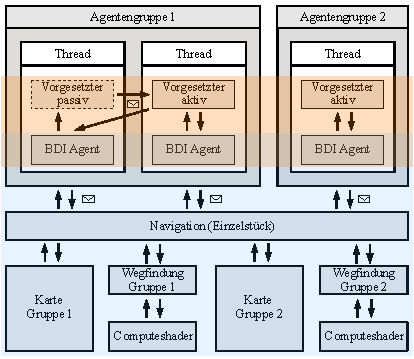
\includegraphics[scale=1.1]{./figures/Architekturdiagramm.pdf}    
     \end{center}
\end{column}
\end{columns}
\end{frame}

\begin{frame}{Agentensystem V1}
\frametitle{Agentensystem V1 -- Wegfindung}
\begin{columns}
\begin{column}{0.7\textwidth}
\begin{block}{Ziel: Ermittlung Entfernungsdaten mit intelligenter Behandlung von Hindernissen für Entscheidungsfindung}
\end{block}
	\begin{itemize}
		\item{50-100 Berechnungen pro Agent und Simulationsschritt}
		\item{CPU-basierte Lösung scheidet aufgrund Zeitbeschränkung aus}
	\end{itemize}
\begin{exampleblock}{Lösung: GPU basierte Wegfindung mittels OpenGL-Computeshader}
\end{exampleblock}
	\begin{itemize}
		\item{bis zu 1.000 Berechnungen pro Simulationsschritt}
		\item{A* Algorithmus mit Heuristik Manhattan-Distanz}
		\item{Herausforderungen im Bereich Speicherkomplexität}
	\end{itemize}
\end{column}
\begin{column}{0.3\textwidth}
    \begin{center}
     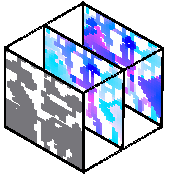
\includegraphics[scale=1.3]{./figures/Pathfinding.pdf}    
     \end{center}
\end{column}
\end{columns}
\end{frame}

\begin{frame}{Agentensystem V1}
\frametitle{Agentensystem V1 -- Ziel- und Absichtsfindung}
\begin{center}
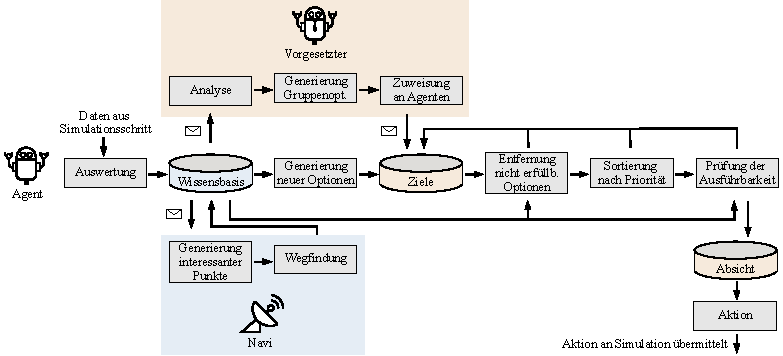
\includegraphics[scale=1.05]{./figures/Entscheidungsfindung2.pdf} 
\end{center}
\end{frame}

\begin{frame}{Agentensystem V1}
\frametitle{Agentensystem V1 -- Verifikation und Problemfindung}
\begin{block}{Validierung}
\begin{itemize}
	\item erfolgt über erreichte Punktzahl in Testspielen
\end{itemize}
\end{block}
\begin{block}{Verifizierung / Problemfindung}
\begin{itemize}
	\item der Wissensbasis über Einzeltests
	\item des Entscheidungsprozesses über punktuelle Einzeltests (Flächendeckende Tests sind aufgrund des dynamischen Systems nicht effizient umsetzbar)
	\item Problemfindung stattdessen über Beobachtungen analog eines Trainers einer Sportmannschaft
\end{itemize}
\end{block}
\end{frame}

\begin{frame}{Agentensystem V1}
\frametitle{Agentensystem V1 -- Grafisches Analysewerkzeug}
\begin{center}
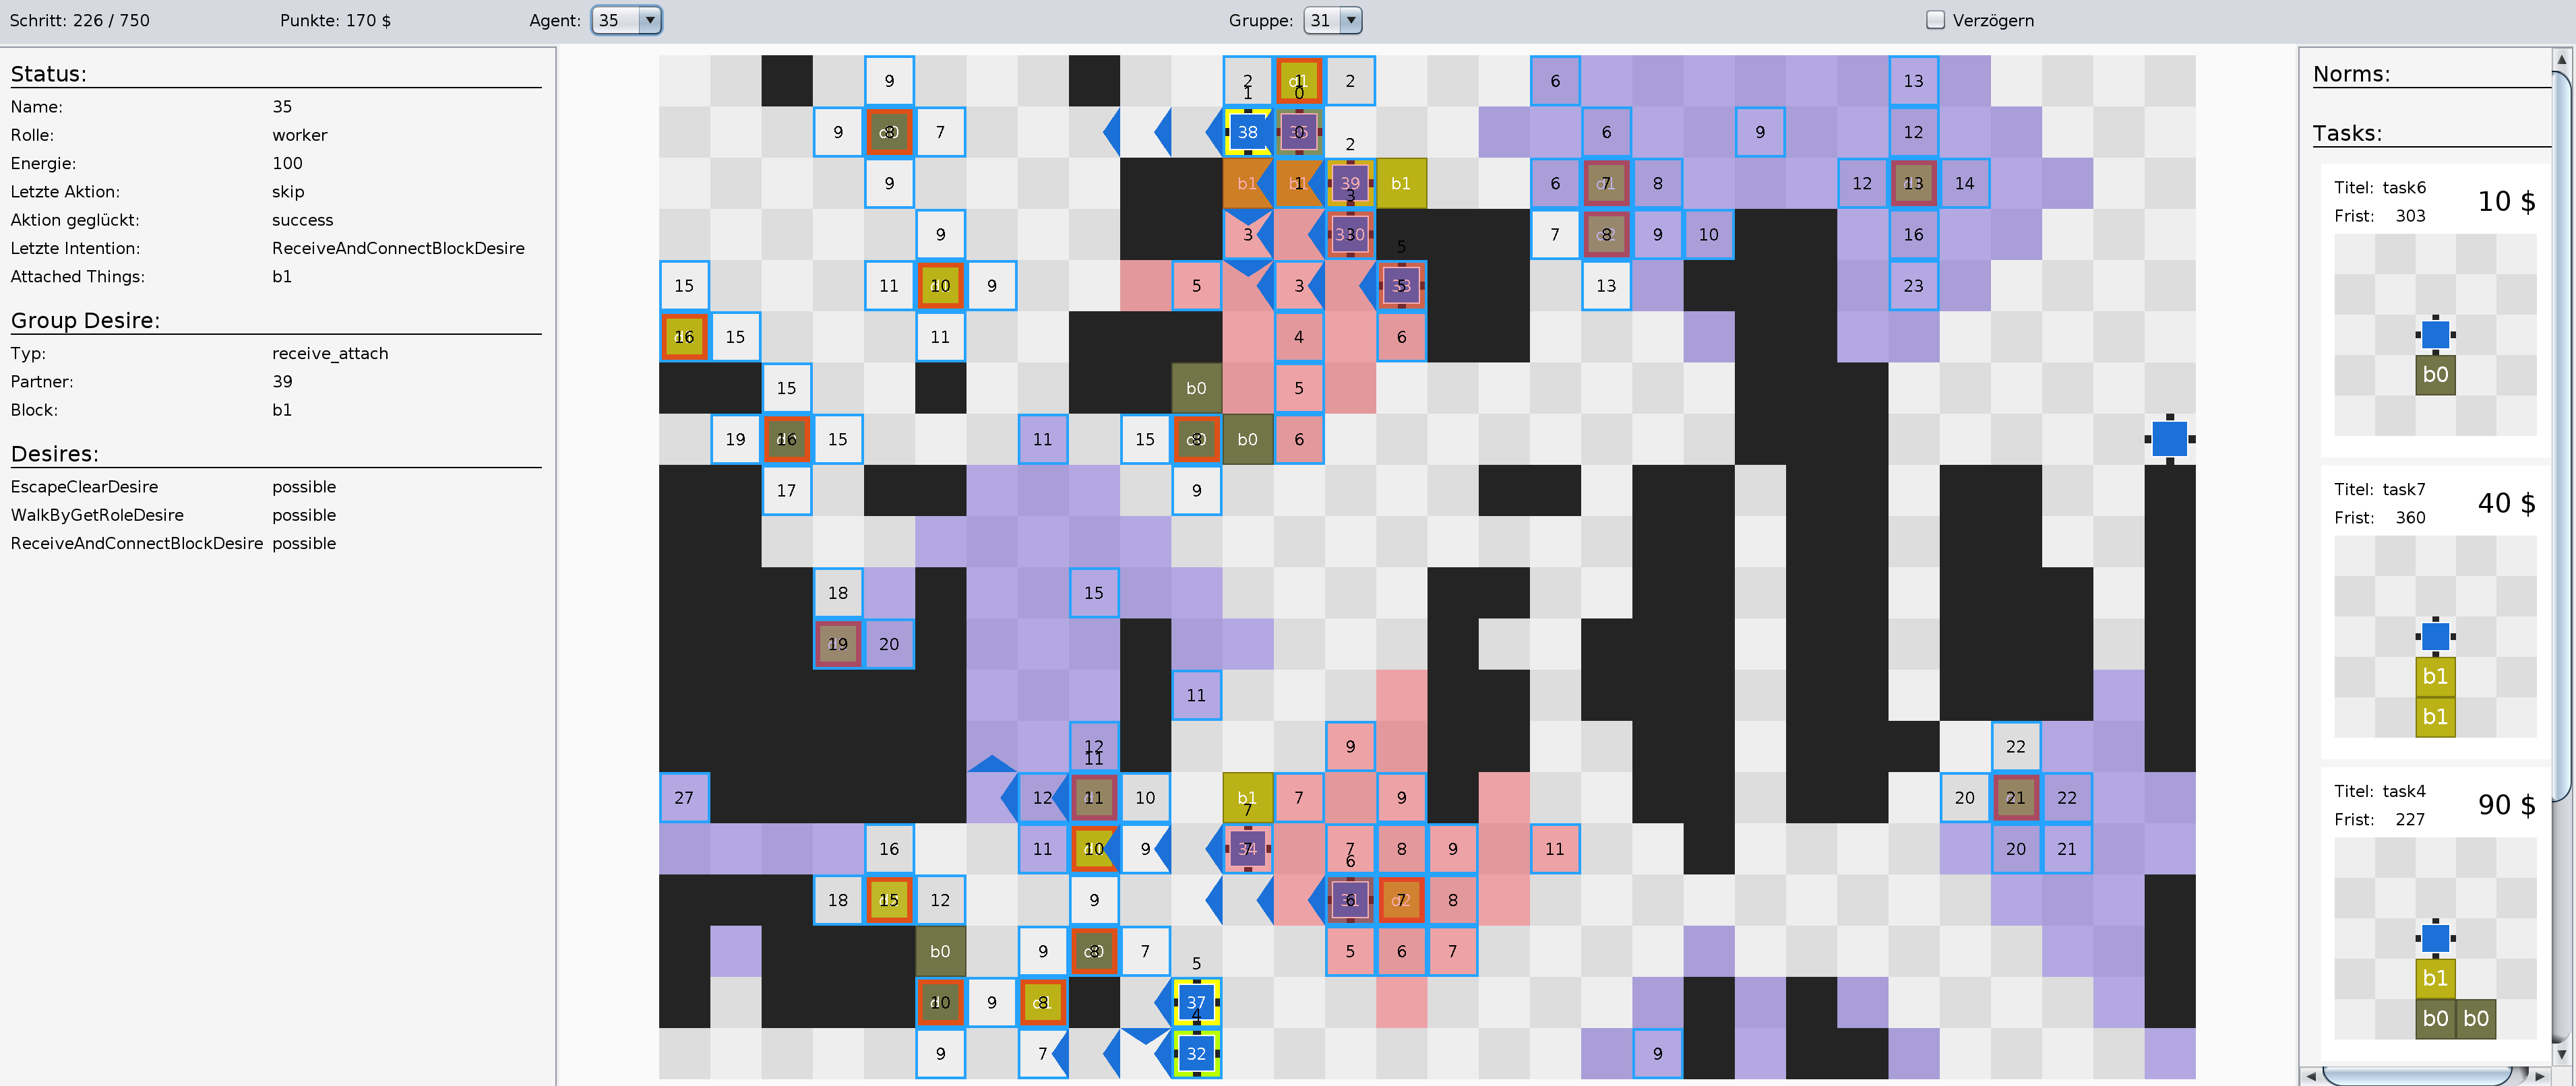
\includegraphics[width=\textwidth]{./figures/Debugger2.png} 
\end{center}
\end{frame}

\section{Agentensystem V2}
\begin{frame}{Agentensystem V2}
	\frametitle{Agentensystem V2}
	\begin{block}{Struktur}
	\end{block}
	\textbf{ }
	\begin{itemize}
		\setlength\itemsep{5mm}
		\item Der AgentV2 arbeitet mit der Step-Methode		
		\item Desires mit und ohne Task-Bezug
	\end{itemize}
	\begin{table}
	\small
	\begin{tabular}{lll}
		\textbf{ohne Task} & \textbf{mit Task} & \textbf{Mehr\-Block\-Task}\\
		LocalExploreDesire & GoAbandonedBlockDesire & MasterMultiBlocksDesire\\
		GoAdoptRoleDesire & GoDispenserDesire & HelperMultiBlocksDesire\\
		ExploreMapSizeDesire & GoGoalZoneDesire & Helper2MultiBlocksDesire\\
		& SubmitDesire & ConnectMultiBlocksDesire\\
	\end{tabular}
	\end{table}
\end{frame}

\begin{frame}{Agentensystem V2}
	\frametitle{Agentensystem V2}
	\begin{block}{Wie finden die Agenten ihre Desires?}
	\end{block}
	\textbf{ }
	\begin{itemize}
		\setlength\itemsep{5mm}
		\item In jedem Step werden alle Desires auf Ausführbarkeit geprüft		
		\item Alle ausführbaren Desires bekommen dynamisch eine Priorität vergeben
		\item Das Desire mit der höchsten Priorität wird zur Intention
		\item Aus der Intention wird die nächste Aktion des Agenten abgeleitet
	\end{itemize}
\end{frame}

\begin{frame}{Agentensystem V2}
	\frametitle{Agentensystem V2}
	\begin{block}{Wie arbeiten die Agenten zusammen?}
	\end{block}
	\textbf{ }
	\begin{itemize}
		\setlength\itemsep{5mm}
		\item Bildung von Supervisor-Gruppen bei jedem Treffen fremder Agenten		
		\item Bildung von dynamischen Adhoc-Kooperationen innerhalb der Supervisor-Gruppen zur Bearbeitung einer Task
		\item Keine zentrale Koordination der Agenten
		\item Steuern der Art und Anzahl der Adhoc-Kooperationen über Setup-Variablen
		\item Nutzung der Adhoc-Kooperationen auch zur Ermittlung der Mapgröße
	\end{itemize}
\end{frame}

\section{Turniere}

\begin{frame}{Turniere}
\frametitle{Turniere}
Teilnahme an Turnier 2-6. \\ Hauptagent war Agent V1 (Agent V2 hat insgesamt 4 Spiele bestritten)
\begin{block}{Turnier 2}
\textcolor{teal}{\smiley{}} max. 370 Punkte über Einzelblockaufgaben (zweiter Platz) \\
\textcolor{red}{\frownie{}} übermäßige Gruppenbildung und gegenseitige Behinderung  
\end{block}
\begin{block}{Turnier 3}
\textcolor{teal}{\smiley{}} max. 720 Punkte über Einzelblockaufgaben (zweiter Platz) \\
\textcolor{red}{\frownie{}} teilweise Gruppenbildung und gegenseitige Behinderung  
\end{block}
\begin{block}{Turnier 4}
\textcolor{teal}{\smiley{}} Mehrblockaufgaben wurden abgegeben \\
\textcolor{teal}{\smiley{}} kaum Gruppenbildung \\
\textcolor{red}{\frownie{}} schlechte Agentenzusammenarbeit (dritter Platz und \textit{nur} max. 680 Punkte)
\end{block}
\end{frame}

\begin{frame}{Turniere}
\frametitle{Turniere}
\begin{block}{Turnier 5}
\textcolor{teal}{\smiley{}} stark verbesserte Agentenzusammenarbeit \\
\textcolor{teal}{\frownie{}} max. 1300 Punkte (erster Platz)  
\end{block}
\begin{block}{Turnier 6}
\textcolor{teal}{\smiley{}} verschärfter Schwierigkeitsgrad wurde gut gemeistert \\
\textcolor{teal}{\smiley{}} Abgabe von Dreiblockaufgaben \\
\textcolor{teal}{\smiley{}} max. 910 Punkte (erster Platz) \\
\end{block}
\begin{block}{Bonusspiel -- Jeder gegen Jeden mit insgesamt 150 Agenten}
\textcolor{teal}{\smiley{}} Agenten blieben performant \\
\textcolor{teal}{\smiley{}} 1370 Punkte (erster Platz)  \\
\textcolor{red}{\frownie{}} Gruppenbildung und gegenseitige Behinderung war zu beobachten
\end{block}
\end{frame}

\section{Rekapitulation}

\begin{frame}{Rekapitulation}
\begin{itemize}
	\item Die umgesetzten Architekturen waren sehr erfolgreich in den Turnieren.
	\item Abgesehen von der Verwendung einer gemeinsamen Wissensbasis fand kaum Austausch zwischen den verfolgten Ansätzen statt, was kritisch zu bewerten ist.
	\item Aufgrund der erreichten Punkte wird vermutet, dass der mehrschichtige Entscheidungsprozess \textit{(Agent V1)} leistungsfähiger ist als der vollständig dezentrale Ansatz \textit{(Agent V2)}
	\item Ein direkter Vergleich ist aber aufgrund der unterschiedlichen Architekturen und Ersteller nur schwer durchzuführen und daher bleibt die Aussage eine Vermutung.
	\item Die Gruppe ist mit der erreichten Funktionalität und deren \\ Qualität zufrieden. Dennoch besteht vielfältiges \\ Verbesserungspotential in der Entscheidungs- und \\Strategiefindung der Agenten.
\end{itemize}
\begin{tikzpicture}[remember picture, overlay]
\node[left] at (current page.-20) 
{
    
\includegraphics[width=0.3\textwidth]{figures/Thanks.pdf}
};
\end{tikzpicture}
\end{frame}


\end{document}
